\documentclass[11pt,a4paper]{article}
\usepackage[margin=25mm]{geometry}
\usepackage{iftex}
\ifPDFTeX\usepackage[T1]{fontenc}\usepackage[utf8]{inputenc}\fi
\usepackage{amsmath,amssymb,graphicx,booktabs,array}
\usepackage[authoryear,round]{natbib}
\usepackage{caption,placeins}
\usepackage[unicode,breaklinks=true,hidelinks]{hyperref}
\setlength{\parindent}{0pt}\setlength{\parskip}{5pt}
\setlength{\emergencystretch}{3em}\setlength{\tabcolsep}{3pt}
\clubpenalty=10000\widowpenalty=10000
\captionsetup{font=small,labelfont=bf}
\newcounter{proposition}
\begin{document}
\begin{center}\Large\bfseries When Is History Long Enough? Conditional Quantile Models versus Historical Rules for Peak Net-Position Limits\end{center}

\begin{abstract}Position limits concern the largest sampled absolute net position during a review period, which an endpoint forecast can miss. We compare historical and conditional quantile forecasts using one FX market maker's positions and aggregate dealer records from the New York Fed and CFTC. Historical rules are difficult to beat across these records, while longer-history FX gains coexist with adverse weekly outcomes and important exceptions. Simulations, learning curves and the partly supported CFTC check are consistent with estimation costs varying with history and shrinkage, while causal attribution remains unresolved. Practical validation should compare scores, breaches and stated limit costs against matched historical benchmarks, since different charges can favor different procedures.\end{abstract}

\noindent\textbf{Keywords:} Peak net positions; Quantile forecasting; Historical benchmarks; Forecast comparison; Calibration; Dealer positions.\par\medskip


\section{Introduction}\label{sec:intro}

Position limits must cover exposure between reviews, since a position that finishes inside a limit can still breach it earlier.
An endpoint forecast therefore answers a different question from a peak forecast, motivating comparisons on the largest sampled absolute net position.

\begin{figure}[htbp]\centering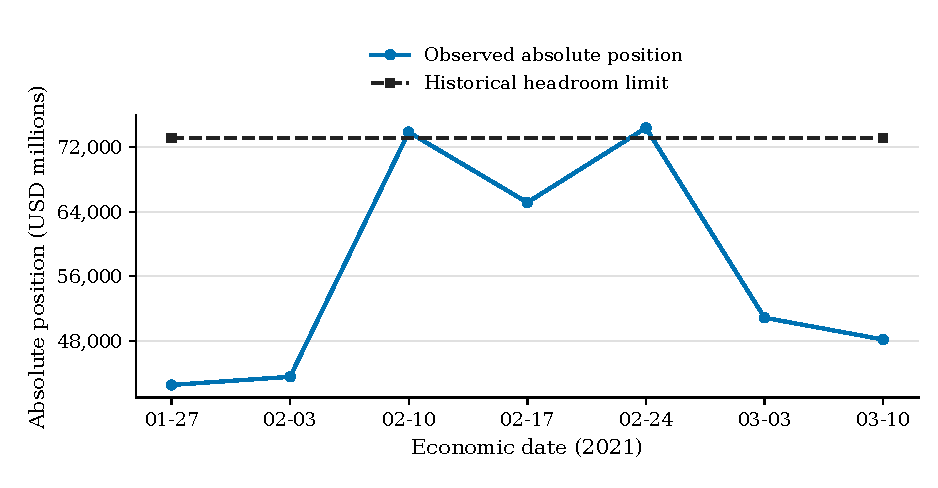
\includegraphics[width=.94\linewidth]{figures/v9-endpoint-peak-example.pdf}
\caption{This Treasury-bill path returns within its reported historical limit at the endpoint, although an earlier position breaches that same limit.
The example follows the earliest eligible original evaluation window, illustrating why endpoint containment can conceal exposure during the review period.}\label{fig:example}
\end{figure}

Conditional models use recent position states and calendar information to adapt a limit, but their estimated relationships consume a finite history.
A historical rule estimates fewer relationships and can remain competitive, making improvement over an explicit historical benchmark the relevant practical question.

We examine one market maker's FX record alongside two official reporting systems that describe different segments of aggregate dealer activity.
New York Fed reports cover government securities, while CFTC categories cover futures markets, requiring distinct targets, scales and historical references.
Both weekly systems report dealer aggregates rather than independent individual dealers, and their economic units and information dates remain distinct.

History, the tested penalty menu and stated limit costs organize the comparisons, while a universal history requirement and causal explanation remain unidentified.
Matched FX gains coexist with adverse weekly comparisons and reversals at the longest tested histories, keeping historical rules a demanding benchmark.

The first contribution connects simulation and FX history patterns with an additional reporting system, extending their comparison while retaining their limits.
Earlier simulations support the registered short-history and long-history loss-sign predictions, while their universal simplification claim fails and FX curves retain reversals.
The new CFTC extension agrees with the short-history counts but misses the registered long-history win target and strict-improvement target.
Its combined verdict is partial agreement, leaving the broader history pattern qualified and a universally sufficient history threshold still unestablished.

The second contribution distinguishes the amount of history from the available procedures, separating candidate performance from the effects of their selection.
An expanded penalty menu removes much of a short-history simulation loss, while financial diagnostics retain selection errors and losses within the finite menu.
The expanded menu includes an ordinary historical quantile, leaving the value of extra predictors unidentified by near-parity performance alone.
Related forecast comparisons leave historical methods alongside many uneliminated alternatives, showing why a single reported winner gives an incomplete account.

The third contribution connects forecast comparisons to stated limit costs, with reserve amounts, breach frequency and exceedance magnitude entering separately.
Their weights can change which tested report is cheaper, although local exceptions persist within the evaluated grid of hypothetical preferences.
The cost comparison illustrates this dependence on preferences, leaving realized funding gains and the effects of trading interventions outside its scope.

Matching training-label histories and refit schedules makes the benchmark explicit, while feature construction and validation can still use different information.
Causal feature effects therefore remain unidentified, and all observed failures, unavailable comparisons and inspected-period qualifications remain part of the evidence.

Section~\ref{sec:target} defines the response and Section~\ref{sec:results} reports the forecasting comparisons, separating matched conditional gains from changes in the reference procedure.
Section~\ref{sec:history-mechanism} connects the history evidence across simulations, FX and CFTC, before Section~\ref{sec:cost} relates these forecast comparisons to stated cost preferences.

\FloatBarrier

\section{Related literature}\label{sec:literature}

Earlier FX studies forecast signed next-hour position intervals using historical states, calendar information and local prediction methods \citep{wisniewski2020,wisniewski2024}. Their chronological training, calibration and test design reports scores and coverage together, providing a natural comparison for the present forecasting task. Our peak response instead uses a complete future path segment and the current magnitude, producing different labels and limits.


Path-risk forecasts address within-period extremes, including MaxVaR's worst cumulative portfolio return under fixed holdings and diffusion assumptions \citep{boudoukh2004}.
The payment-liquidity thesis forecasts conditional maximum deficits from confidential transactions, while settlement studies examine tail liquidity needs and collateral requirements \citep{hoogen2017,petrunia2019,arjani2020}.
Duffie and colleagues study dealer capacity and Treasury-market functioning, including PnL quantile forecasts; these responses differ from the sampled absolute-position peak \citep{duffie2023}.


Regression quantiles target asymmetric forecast errors directly \citep{koenker1978}, while autoregressive quantiles and quantile forests supply other conditioning structures \citep{engle2004,meinshausen2006}. Consistent scores and elementary-score representations permit comparisons across evaluation preferences, rather than selecting a forecast solely from its apparent coverage \citep{gneiting2011,ehm2016}.
The extended literature matrix compares these earlier responses with the present sampled peak, its completed labels and matched historical controls.




The matched FX gain changes interpretation with its reference, while the weekly comparisons expose both tuning errors and finite-menu losses. Expanded simulation menus remove large short-history losses, while parameter switching misses its registered extra-loss criterion, leaving that switching effect unidentified. Higher reserve charges and lower fixed breach charges generally favor regression in CFTC, although local exceptions remain. Paired tests provide the statistical framework for these forecast comparisons, while inventory-sensitive quoting motivates the underlying problem of monitoring exposure \citep{dm1995,gw2006,mcs2011,avellaneda2008}. These findings concern passive reports on observed position paths, leaving their effect on subsequent trading decisions unmeasured.

\FloatBarrier

\section{The forecast target}\label{sec:target}

The target is the largest sampled absolute position from issue time through the stated horizon, with \(N_t\) denoting signed position and \(\mathcal F_t\) the issue-time information. The peak \(Y_{t,H}\), observed floor \(B_t\) and nonnegative headroom \(Z_{t,H}\) satisfy the following identities.


\[
Y_{t,H}=\max_{0\le h\le H}|N_{t+h}|,\qquad B_t=|N_t|,\qquad Z_{t,H}=Y_{t,H}-B_t\ge0.
\]

A feasible limit covers the current observed exposure, but Figure~\ref{fig:example} shows that endpoint containment can still conceal an earlier breach. We score reports with pinball loss and count a strict breach when the peak exceeds the limit.


\[
\rho_\tau(u)=\tau u_+ +(1-\tau)(-u)_+,\qquad I_{t,H}=\mathbf 1\{Y_{t,H}>C_{t,H}\}.
\]

\refstepcounter{proposition}\noindent\textbf{Proposition~\theproposition{} (known-floor projection).}\label{prop:floor} Suppose \(Y\ge B\) almost surely and the issue information contains \(B\). Projecting any forecast \(c\) to \(\max\{B,c\}\) weakly improves pinball loss for every outcome, with the gain shown below. The true conditional lower inverse quantile at level \(1-\alpha\) has strict exceedance probability at most \(\alpha\), including at atoms.


\[
\rho_\tau(Y-c)-\rho_\tau(Y-\max\{B,c\})=\tau(B-c)_+,\qquad \Pr(Y>q\mid\mathcal F_t)\le\alpha.
\]

\refstepcounter{proposition}\noindent\textbf{Proposition~\theproposition{} (classical endpoint-to-peak bound).}\label{prop:levy} Let future real increments be independent and individually symmetric about zero, with partial sums \(S_h\). Fix a starting position \(x\), set \(B=|x|\), and let \(q\) be the population \((1-\alpha/2)\) quantile of \(|S_H|\). The triangle inequality and the classical L\'evy maximal inequality imply the bound below. A conditional application requires these assumptions and the endpoint quantile under the law given issue-time information.


\[
\Pr\!\left(\max_{0\le h\le H}|x+S_h|>B+q\right)\le\Pr\!\left(\max_h|S_h|>q\right)\le2\Pr(|S_H|>q)\le\alpha.
\]

Supplement Sections S1--S2 retain the proofs and empirical qualifications, while \href{https://github.com/ByronLi0207/financial-mathematics-paper-20261020/blob/final-jof/EXTENDED_RESULTS.md}{the original full Supplement: Sections S3--S5} distinguish mean-reverting levels from serially correlated increments.


Separately fitted horizons can violate the ordering of a common lower-inverse peak quantile under the same information law. Sorting crossed reports weakly improves equally weighted aggregate pinball loss when units and quantile levels coincide. The guarantee concerns aggregate pinball loss under those conditions; individual horizons, other weighting schemes and coverage retain their separate qualifications.
The Supplement preserves the original crossing diagnostic and precise analytic conditions, including the requirement for a common lower-inverse quantile convention.


\FloatBarrier

\section{Data}\label{sec:data}

The FX application uses the hourly Net Position Time Series Dataset, reporting market-maker client-flow positions \citep{dataset,wisniewski2020}. Its 18,576 records retain source USD units; the later, earlier and full-prefix comparisons use distinct chronological issue grids with the same sampled-peak definition.

The weekly data are New York Fed Primary Dealer Statistics, whose reporting definitions follow the government-securities dealer framework and position-accounting instructions \citep{nyfeddata,fr2004_2013,fr2004_2024}. The Treasury-bill series has 706 economic-date observations in USD millions, measuring fair-value positions aggregated as long-minus-short totals. Additional categories pass metadata and calendar checks and use complete weekly grids, with separate fits by category.

Daily aggregation takes the last recorded position on each nonempty source-naive calendar day, retaining partial boundary days in the observed series.
It yields 930 days and 501 common evaluation dates, with each completed day's end serving as the time of the forecast.
The resulting daily target is a peak over subsequent daily records, so aggregation changes both the measurement clock and the sampled response.

The CFTC application retrospectively evaluates a survivor universe using downloaded economic dates and futures-only Dealer/Intermediary long positions minus short positions \citep{cftcTFF}. The fixed screen requires uninterrupted report weeks from 2010, stable literal codes, exchange and units. It excludes documented consolidation-code families before ranking eligible contracts by full-sample mean open interest. Seventeen contracts pass the screen, below the planned maximum of twenty. Supplement Section S10 lists every selected code and explains the eligibility rules; complete code-level exclusions remain linked there.
Full-sample eligibility makes this universe a retrospective comparison choice, rather than a universe that a forecaster could have selected prospectively.

The retained CFTC series contains 877 weekly positions, with a common observation grid used to align forecasts across every selected contract.
Its final position date is 20 October 2026, which also completes the final sampled peak used in the evaluation.

Validation uses 52 forecast dates, while evaluation retains the last 260 eligible dates under the inherited chronological design and market universe.
The horizon spans six subsequent records, maintaining the same target across the older comparisons and the new mechanism extension.
The evaluation position grid begins on 21 September 2021, after the validation labels have completed under the stipulated information convention.
Its final forecast position date is 8 September 2026, leaving the required future records for completion of the peak label.
Refits occur every thirteen records, using downloaded economic dates and preserving the distinction between recorded positions and historical public availability.
The original training histories contain 52 and 260 records, while first-release vintages remain unobserved throughout these retrospective comparisons.
The registered extension adds a 520-week history on the same evaluation dates, retaining the older histories and their saved reports unchanged.
Positions usually refer to Tuesday and are released Friday, so the recorded position clock differs from the public information clock.

Table~\ref{tab:v12-data} describes the aligned source records and complete six-record peaks, with monetary series expressed in USD millions. Panel summaries take nine separate medians of within-series statistics, preserving the heterogeneous exposure units across categories and contracts. Within each forecasting comparison, every method uses identical peak labels, current floors and forecast dates, keeping its reported target and comparison grid aligned. The same-record FX aggregation holds dealer identity fixed while changing its measurement clock and sampled response.

\begin{table}[!htbp]
\centering
\caption{Data and matched six-record peak summaries.}\label{tab:v12-data}
\begingroup\fontsize{7.5}{9}\selectfont\setlength{\tabcolsep}{2pt}
\textit{Panel A. Sources, aligned samples and existing split dates}\\[3pt]
\begin{tabular}{@{}lllllll@{}}
\toprule
Data & Frequency & Series / records & Unit & Sample & Validation & Evaluation \\
\midrule
FX, hourly & Hourly & 1 / 18,576 & USD mn & 2014-02 to 2017-01 & 2015-10 to 2015-12 & 2016-01 to 2017-01 \\
FX, daily & Day end & 1 / 930 & USD mn & 2014-02 to 2017-01 & 2015-02 to 2015-04 & 2015-05 to 2016-12 \\
Treasury bills & Weekly & 1 / 706 & USD mn & 2013-04 to 2026-10 & 2019-07 to 2020-07 & 2021-01 to 2026-04 \\
NY Fed panel & Weekly & 12 / 706 & USD mn & 2013-04 to 2026-10 & 2019-07 to 2020-07 & 2021-01 to 2026-04 \\
CFTC panel & Weekly & 17 / 877 & Contracts & 2010-01 to 2026-10 & 2020-08 to 2021-08 & 2021-09 to 2026-09 \\
\bottomrule
\end{tabular}
\par\vspace{7pt}
\textit{Panel B. Within-series mean, sample SD and empirical 95th percentile}\\[3pt]
\begin{tabular}{@{}ll*{9}{r}@{}}
\toprule
 & & \multicolumn{3}{c}{$|N|$} & \multicolumn{3}{c}{Peak $Y$} & \multicolumn{3}{c}{Headroom $Z$} \\
\cmidrule(lr){3-5}\cmidrule(lr){6-8}\cmidrule(lr){9-11}
Data & Unit & Mean & SD & 95th & Mean & SD & 95th & Mean & SD & 95th \\
\midrule
FX, hourly & USD mn & 8.92 & 10.2 & 27.6 & 11.1 & 11.7 & 30.2 & 2.15 & 5.92 & 7.96 \\
FX, daily & USD mn & 9.00 & 10.5 & 27.5 & 17.9 & 16.6 & 41.0 & 8.91 & 14.8 & 24.9 \\
Treasury bills & USD mn & 39,500 & 27,200 & 92,600 & 55,300 & 30,400 & 108,000 & 15,800 & 16,000 & 50,000 \\
NY Fed panel & USD mn & 12,400 & 8,340 & 33,300 & 16,000 & 9,040 & 37,400 & 3,750 & 3,560 & 10,500 \\
CFTC panel & Contracts & 60,200 & 46,000 & 148,000 & 81,800 & 45,600 & 169,000 & 19,900 & 20,900 & 60,600 \\
\bottomrule
\end{tabular}
\endgroup
\begin{minipage}{.98\linewidth}\footnotesize\emph{Notes.} Records are per series; complete $H=6$ peak counts are 18,570, 924, 700, 700 and 871, respectively, including the issue anchor. Earlier hourly FX validation spans 2015-04 to 2015-07 and evaluation spans 2015-07 to 2015-10; daily FX uses each nonempty source-naive day\textquotesingle s last record, and both FX periods had been inspected. SD uses $m-1$ and the empirical 95th percentile has rank $\lceil95m/100\rceil$; dollar values are in millions, panel entries are separate within-series medians without exposure pooling, and CFTC retains heterogeneous native contract counts.\end{minipage}
\end{table}


\FloatBarrier

\section{Forecasting methods}\label{sec:methods}

Unless otherwise stated, forecasts target the conditional quantile at \(\tau=19/20\). The horizons \(H\in\{6,24\}\) count subsequent source records, and each peak includes the issue position. Calendar gaps extend an FX horizon's elapsed span, while weekly and daily steps represent different review intervals under the same nineteen-to-one error-weight preference.

Historical headroom adds a corrected empirical quantile of completed headrooms to the observed magnitude:
\[
F_{t,H}=B_t+Q_j\{Z_{i,H}:i\in\mathcal T_r\},\qquad
j=\lceil(m+1)\tau\rceil,\quad m=|\mathcal T_r|.
\]
Here \(Q_j\) is the \(j\)th order statistic, and the training set contains only labels completed by refit time \(r\).
At the sensitivity level where this rank exceeds the sample size, the rank is capped at \(m\), producing the historical maximum.
Coverage under the observed dependence remains unguaranteed by this finite-sample reporting convention, even though its completed-label ranking is precisely defined. In weekly replays, the current floor is known under the stipulated economic-date information set of the downloaded vintage. Historical first-release availability remains unreconstructed, qualifying the information interpretation separately from the mathematical guarantee for a floor already known at issue time.
Translated paths reanchor historical signed paths before computing their peaks, while historical-peak quantiles are projected to the same observed floor. The endpoint plug-in uses an absolute-displacement quantile; Table~\ref{tab:methods} gives the executed menus and schedules.

Ridge quantile regression links completed headroom labels to issue-known position states and calendar variables. Full regression uses 33 predictors plus an unpenalized intercept, allowing position states and calendar variables to enter the conditional report.
Its four-feature variant uses magnitude, signed level and paired short- and long-window root mean square (RMS) increment measures of recent changes.
Standardization uses only training rows with completed labels, keeping the feature transformation tied to the data available for that fit. Expanded-menu full regression changes only the penalty grid, using the following training-scaled objective:
\[
(\hat a,\hat b)=\arg\min_{a,b}\left\{
\frac1m\sum_{i\in\mathcal T_r}\rho_\tau\!\left(\frac{Z_{i,H}}s-a-x_i^\top b\right)
+\frac\lambda2\|b\|_2^2\right\},\qquad
\lambda\in\{0.001,0.01,0.1,1,10,\infty\}.
\]
The intercept is unpenalized; training rows alone determine the feature transform and response scale \(s\).
Reports are \(B_t+s\max\{0,\hat a+x_t^\top\hat b\}\), while infinite shrinkage gives the ordinary empirical headroom quantile.
The original menus and scale definitions remain in Table~\ref{tab:methods} and Supplement Sections S3 and S5.

Local quantiles use neighboring historical states, with an increment-scaled variant, while quantile forests use the training observations represented in their leaves \citep{meinshausen2006}.
Filtered paths simulate positions from GARCH-standardized empirical innovations drawn independently with replacement, and tail methods fit volatility-scaled headroom \citep{hull1998,barone1999,mcneilfrey2000}. \href{https://github.com/ByronLi0207/financial-mathematics-paper-20261020/blob/final-jof/EXTENDED_RESULTS.md}{The original full Supplement: Sections S7 and S11--S18} report benchmark results and failures; Section S13 links the complete legacy inventories.

Further comparisons apply delayed calibration, fixed combinations and conservative selection to the same peak response. A headroom CAViaR recursion and calibration wrappers follow existing methods, with calibration parameters updating only after the corresponding outcomes mature \citep{engle2004,gibbs2021}.
Fixed mean and median combinations use predefined members, preserving their original composition separately from the rules that select a single procedure. Conservative selection favors the strongest shrinkage whose validation loss is within one paired HAC standard error of the winner's loss. This adapts one-standard-error selection \citep{hastie2009} to paired forecast losses.

\begin{table}[htbp]\centering\small
\caption{Forecast definitions and executed menus retain the original procedure codes, connecting each reported comparison to its saved result files.
Matched training-label histories and update schedules make the reference explicit, while the Supplement preserves the full normalization and parameter conventions.}\label{tab:methods}
\begin{tabular}{>{\raggedright\arraybackslash}p{2.9cm}>{\raggedright\arraybackslash}p{6.0cm}>{\raggedright\arraybackslash}p{5.3cm}}\toprule
Method & Forecast definition & Executed menu / setting\\\midrule
Historical headroom (F) & Current floor plus a quantile of completed peak headrooms & Original FX histories \{720,2880\}; weekly \{52,260\}\\
Translated path (S) & Translate completed signed paths to the current position before taking their peaks & Same completed training targets; fixed-window and rolling-window controls\\
Historical peak (K) & Historical absolute-peak quantile projected to the current floor & Same histories and update controls\\
Quantile regression (QR) & Training-scaled headroom regression with ridge slopes and an unpenalized intercept & Original three-point menu; six-point menu $\{0.001,0.01,0.1,1,10,\infty\}$\\
Local quantiles (KNN) & Neighbor headroom quantile, with a separate increment-scale variant & Training-only transforms and fixed neighbor menus; Supplement Sections S3 and S5\\
Four-feature regression (QR4) & Current signed/magnitude positions and short/long increment RMS & Original five-point menu; six-point paired comparison below\\
Endpoint plug-in (L) & Floor plus a high absolute-displacement endpoint quantile & Proposition~\ref{prop:levy}; empirical plug-in evaluated separately\\
Further benchmarks & Autoregressive replay; filtered paths; peak-tail fit; quantile forest & Existing bounded specifications; results and complete failures linked from \href{https://github.com/ByronLi0207/financial-mathematics-paper-20261020/blob/final-jof/EXTENDED_RESULTS.md}{the original full Supplement: Sections S7 and S34}\\
Coverage and combinations & Delayed projected ACI-style wrappers; headroom SAV; fixed forecast combinations & Original-source wrapper/SAV inventory and broader combination inventory are separate\\
\bottomrule\end{tabular}
\par\smallskip\begin{minipage}{.98\linewidth}\footnotesize Training histories count completed labels, and fixed-window models refit every 24 FX records or 13 weekly records under their original schedules. Quantile and normalization conventions are detailed in Supplement Sections S3 and S5; this table retains the executed menus. The CFTC mechanism extension adds the longer history described in Section~\ref{sec:history-mechanism}.\end{minipage}
\end{table}

\FloatBarrier

\section{Evaluation design}\label{sec:evaluation}

At refit time \(r\), only labels satisfying \(i+H\le r\) are eligible; predictors use issue-known observations and training transforms remain fixed until the next refit. Original comparisons select parameters in the preceding validation segment, while the full-prefix backcast holds its specified penalties fixed. Original weekly comparisons use 52 outer validation origins with overlapping labels.

Matched comparisons hold the completed-response history and refit schedule fixed for regression and historical headroom. The main FX reference uses a shorter rolling history, whereas the main Treasury reference shares regression's longer history and refit schedule. Tables~\ref{tab:fx} and~\ref{tab:weekly} report both alongside the other comparison sets.

Accuracy uses mean pinball loss and breaches are strict peak exceedances, scoring passive reports along the observed position paths. Paired loss differences use HAC covariance with the horizon-based bandwidth rule \citep{dm1995,nw1987}. Tables identify the small-sample adjustment and named multiplicity families \citep{hln1997,holm1979}. Hit diagnostics use a fixed spaced grid and condition the transition likelihood on its initial hit \citep{kupiec1995,christ1998}.
For paired loss differences \(d_t\), the comparison statistic and its existing bandwidth are
\[
\mathrm{DM}=\frac{\sqrt n\,\bar d}{\sqrt{\widehat\Omega_K}},\qquad
K=\min\{n-1,\max[H,\lfloor4(n/100)^{2/9}\rfloor]\},
\]
where \(\widehat\Omega_K\) is the Newey--West long-run variance estimate with Bartlett weights.


\subsection{Inspected periods limit the scope of confirmation}

The original protocol fixes the two main comparisons and their reference procedures; the original FX evaluation period had already been inspected. Each new analysis states its prediction thresholds before computation (Supplement Section S15), with chronological records retained separately from the results. These later checks remain retrospective, and their descriptive fractions do not treat related markets as independent replications.

\subsection{Joint comparisons retain statistically unseparated procedures}

A model confidence set contains the procedures a joint loss comparison does not eliminate under its stated statistical approximation. We form a 90\% model confidence set separately for each complete source, period, horizon and history grid \citep{mcs2011}. The range statistic uses 1,000 stationary-bootstrap replications, retaining the original implementation and its approximation to dependence among the paired losses.
Its recorded software version is arch 8.0.0, with the precise implementation retained alongside the saved comparison results and execution records.
The block length is $\max\{H,\lceil n^{1/3}\rceil\}$, preserving the inherited dependence convention rather than selecting a new setting after observing these comparisons. All complete saved procedures enter on matching origin grids and targets, while incomplete prior methods remain explicitly unavailable. The nominal level presumes suitable loss dependence and leaves earlier research-stage model development outside the stated uncertainty calculation for each comparison.

Exact duplicate loss columns enter the bootstrap once, and their procedure labels are restored afterward. Historical reports are merged only after their full forecasts and targets match, while rolling references remain distinct. Several methods can produce identical losses, allowing a surviving loss pattern to represent multiple distinct procedures whose labels remain explicitly listed.
The reported fractions summarize related tasks descriptively, with independent cross-market significance outside the scope of the fixed bootstrap exercise.

\FloatBarrier

\section{Results}\label{sec:results}

\subsection{Matched FX gains depend on the reference}

Long-history FX regression beats matched historical headroom in both periods, yet its ranking against the shorter rolling reference reverses in the earlier period (Table~\ref{tab:fx}). The reference procedure is therefore part of the substantive finding, with a matched conditioning gain leaving the ranking against other historical rules unresolved.

Beyond the matched long-history case, short-history FX regression performs poorly at the longer horizon. Loss rises by 31.5\% against matched historical headroom. Regression records 924 breaches against 427 for the reference; the full horizon map retains the other adverse comparisons. This adverse case confines the interpretation of the matched long-history gain to its evaluated horizon and training-window setting, retaining the broader failures.

Delayed calibration retains the later matched FX gain, although its breach count remains slightly higher than wrapped historical headroom on common origins (Table~\ref{tab:fx}). Calibration therefore changes breach frequency, while the distinct score and hit rankings persist on the common comparison grid. Each wrapper has a higher saved mean score than its own unwrapped base, so the retained relative ranking coexists with an absolute score cost. The headroom-SAV recursion refits on its evaluation training pools, whereas the selected ACI wrapper carries its delayed calibration state.

\href{https://github.com/ByronLi0207/financial-mathematics-paper-20261020/blob/final-jof/EXTENDED_RESULTS.md}{The original full Supplement: Sections S20--S21 and S26} report the state, target-level and overlapping full-prefix comparisons (\href{https://github.com/ByronLi0207/financial-mathematics-paper-20261020/blob/final-jof/EXTENDED_RESULTS.md}{the original full Supplement: Tables S19--S21 and S25--S26}).

\begin{table}[htbp]\centering\small
\caption{Long-history short-horizon FX regression is compared under two references across the earlier and later evaluation periods retained in the study.
Negative percentages favor regression, revealing recurring matched gains alongside a reversal in its comparison with the shorter rolling historical reference.}\label{tab:fx}
\begin{tabular}{>{\raggedright\arraybackslash}p{2.6cm}>{\raggedright\arraybackslash}p{4.4cm}>{\raggedleft\arraybackslash}p{2.5cm}>{\raggedleft\arraybackslash}p{1.5cm}>{\raggedright\arraybackslash}p{3.2cm}}\toprule
Period / procedure & Reference & Loss change (\%) & Issues & Strict breaches (regression / reference)\\\midrule
Later / original main comparison & Shorter-history rolling headroom & -12.66 & 6625 & 376 / 332\\
Later / matched & Same-history fixed-window headroom & -14.77 & 6625 & 376 / 360\\
Earlier / original structure & Shorter-history rolling headroom & +3.17 & 1440 & See complete earlier-period tables\\
Earlier / matched & Same-history fixed-window headroom & -16.62 & 1440 & 20 / 16\\
Later / coverage-wrapped & Same-history wrapped headroom & -15.00 & 6625 & 329 / 328\\
\bottomrule\end{tabular}
\par\smallskip\begin{minipage}{.98\linewidth}\footnotesize Regression uses history 2880 and horizon 6, retaining the original comparison grid for each period reported in this table.
The original rolling reference uses 720 observations, making its available history shorter than the matched historical headroom reference used alongside regression.
The earlier matched comparison uses the original three-penalty regression, while the later one-standard-error rule remains a separate selection exercise.
The wrapper comparison is a separate finite projected delayed ACI-style exercise, using its common evaluation dates and inherited calibration design.\end{minipage}
\end{table}

\FloatBarrier
\subsection{FX history gains reverse within the tested range}\label{sec:fx-history}

History sensitivity within the original FX record reverses across the tested grid, as full regression gives back gains at the longest history. Section~\ref{sec:history-mechanism} combines both horizon curves
with the simulation and CFTC evidence, retaining every tested window and its
own matched historical reference.

\FloatBarrier

\subsection{Historical rules remain competitive across reporting clocks}

The reference-sensitive hourly results motivate comparisons with other measurement clocks and reporting systems, each retaining matched histories and completed peak labels.

At weekly frequency, the Treasury-bill comparison favors historical headroom on both accuracy and breaches, extending the adverse ranking beyond the hourly examples. The earlier short-window version retains its separate adverse result because it uses a different history (Table~\ref{tab:weekly}).

Stronger regularization narrows weekly panel losses but leaves historical rules ahead, with conservative selection choosing the intercept-only report in 17 of 26 earlier cells (Table~\ref{tab:weekly}). Its largest relative loss increase occurs in the Treasury-bill short-history, 24-step comparison, despite conservative selection.

Simpler conditioning and fixed combinations retain adverse weekly comparisons, reinforcing the importance of an explicit historical benchmark for each forecast setting. \href{https://github.com/ByronLi0207/financial-mathematics-paper-20261020/blob/final-jof/EXTENDED_RESULTS.md}{The original full Supplement: Sections S16--S18} retain their complete losses and failures, including the headroom-recursion results (\href{https://github.com/ByronLi0207/financial-mathematics-paper-20261020/blob/final-jof/EXTENDED_RESULTS.md}{the original full Supplement: Tables S14--S17}).

Returning to the same FX record, historical headroom wins seven of eight daily comparisons, retaining a demanding reference after changing the measurement clock.
The exception uses four predictors, with its complete specification and matched historical comparison retained alongside the adverse cases in the Supplement.
Its training history is 260 and its horizon is 6, maintaining common completed targets and forecast dates across the matched procedures.
The regression loss falls by 3.0\%, although this accuracy gain accompanies a worse breach count than the matched historical report.
Regression records 37 breaches versus 30 for headroom, preserving the score--breach disagreement while aggregation changes the leading method in most comparisons.

\begin{table}[htbp]\centering\small
\caption{Weekly evidence combines the original main comparison, added panel and earlier-period comparisons, with counts referring to related tasks rather than independent dealers.
Stronger regularization narrows the losses of conditional procedures while leaving substantial failures, including the adverse bill comparison under conservative selection.}\label{tab:weekly}
\begin{tabular}{>{\raggedright\arraybackslash}p{4.3cm}>{\raggedright\arraybackslash}p{4.7cm}>{\raggedleft\arraybackslash}p{2.7cm}>{\raggedright\arraybackslash}p{2.5cm}}\toprule
Comparison set & Procedure & Loss change / median (\%) & Higher-loss cells\\\midrule
Original Treasury-bill main comparison & Original regression, long history & +50.79 & Original main comparison\\
Earlier Treasury-bill short-window version & Short-history short-window version & +144.30 & Different history\\
Additional panel & Original full regression & +92.63 & 45 / 48\\
Additional panel & Four-feature regression & +9.91 & 37 / 48\\
Additional panel & Full regression, expanded penalties & +9.22 & 34 / 48\\
Additional panel & Ordinary empirical headroom quantile & +0.50 & 30 / 48\\
Earlier weekly groups & Validation-minimum expanded rule & +4.15 & 26 groups\\
Earlier weekly groups & One-standard-error rule & +5.37 & 26 groups\\
\bottomrule\end{tabular}
\par\smallskip\begin{minipage}{.98\linewidth}\footnotesize The original bill main comparison has 54 versus 28 strict breaches, favoring the historical report alongside its lower mean loss.
Its evaluation contains 277 forecast dates, with the complete paired results retained under the original chronological design and target definition. Earlier short-history bill results use a different history; the one-standard-error worst excess is +181.39\%, and all its prewritten success criteria remain unmet. \href{https://github.com/ByronLi0207/financial-mathematics-paper-20261020/blob/final-jof/EXTENDED_RESULTS.md}{The original full Supplement: Sections S11--S15} list all panel and selection results (\href{https://github.com/ByronLi0207/financial-mathematics-paper-20261020/blob/final-jof/EXTENDED_RESULTS.md}{the original full Supplement: Tables S9--S13}).\end{minipage}
\end{table}

\subsubsection{CFTC repeats the benchmark pattern across markets}

The independent reporting system gives a similar overall ranking: a historical headroom rule has lower loss in 29 of 34 contract/history comparisons. This meets the pre-specified 60\% threshold, using the better realized score of corrected and ordinary empirical historical reports rather than an executable selector. Corrected historical headroom remains the fixed matched reference, with the ordinary empirical version reported separately. Both full-regression medians exceed the pre-specified ten-percent tolerance, whereas four-feature regression moves closer to history with the longer window. These comparisons extend the benchmark pattern to a separate reporting system while retaining substantial contract-level variation.
This older reference comparison differs from Section~\ref{sec:history-mechanism}, whose new history predictions use fixed corrected-rank headroom and separately registered thresholds.





\subsubsection{Historical methods remain in most joint comparison sets}

Joint comparison leaves matched historical methods alongside alternatives in most sets, with a single historical method surviving in only a small minority. These results support retaining historical controls while leaving many alternatives uneliminated under the fixed bootstrap approximation. Surviving procedures remain statistically unseparated under the specified comparison, while equality of their predictive risks remains a stronger, unestablished proposition.
Table~\ref{tab:v10-mcs-main} reports surviving methods, and Supplement Section S11 retains every set, method p-value, identical-loss class and prior unavailable method.

\begin{table}[!htbp]\centering\footnotesize
\setlength{\tabcolsep}{4pt}
\caption{Ninety-percent model confidence sets across all planned comparisons. Counts retain their comparison or conditional-procedure denominators.}\label{tab:v10-mcs-main}
\begin{tabular}{lrrrrr}\toprule
Group & Complete & Matched history & Sole historical & Conditional & Unavailable \\
 & / planned & included & method & excluded & procedures \\ \midrule
FX original & 4/4 & \makebox[3.2em][r]{2/4} (\makebox[2.9em][r]{50.0}\%) & \makebox[3.2em][r]{0/4} (\makebox[2.9em][r]{0.0}\%) & \makebox[3.2em][r]{39/66} (\makebox[2.9em][r]{59.1}\%) & 6 \\
FX earlier period & 4/4 & \makebox[3.2em][r]{3/4} (\makebox[2.9em][r]{75.0}\%) & \makebox[3.2em][r]{0/4} (\makebox[2.9em][r]{0.0}\%) & \makebox[3.2em][r]{1/15} (\makebox[2.9em][r]{6.7}\%) & 2 \\
Treasury bills & 4/4 & \makebox[3.2em][r]{4/4} (\makebox[2.9em][r]{100.0}\%) & \makebox[3.2em][r]{0/4} (\makebox[2.9em][r]{0.0}\%) & \makebox[3.2em][r]{11/74} (\makebox[2.9em][r]{14.9}\%) & 4 \\
Other NYFed panels & 48/48 & \makebox[3.2em][r]{46/48} (\makebox[2.9em][r]{95.8}\%) & \makebox[3.2em][r]{0/48} (\makebox[2.9em][r]{0.0}\%) & \makebox[3.2em][r]{110/384} (\makebox[2.9em][r]{28.6}\%) & 48 \\
Same-record daily FX & 4/4 & \makebox[3.2em][r]{4/4} (\makebox[2.9em][r]{100.0}\%) & \makebox[3.2em][r]{2/4} (\makebox[2.9em][r]{50.0}\%) & \makebox[3.2em][r]{5/8} (\makebox[2.9em][r]{62.5}\%) & 0 \\
CFTC & 34/34 & \makebox[3.2em][r]{31/34} (\makebox[2.9em][r]{91.2}\%) & \makebox[3.2em][r]{0/34} (\makebox[2.9em][r]{0.0}\%) & \makebox[3.2em][r]{31/136} (\makebox[2.9em][r]{22.8}\%) & 0 \\
All comparisons & 98/98 & \makebox[3.2em][r]{90/98} (\makebox[2.9em][r]{91.8}\%) & \makebox[3.2em][r]{2/98} (\makebox[2.9em][r]{2.0}\%) & \makebox[3.2em][r]{197/683} (\makebox[2.9em][r]{28.8}\%) & 60 \\
\bottomrule\end{tabular}
\par\smallskip\begin{minipage}{.98\linewidth}\footnotesize
Matched history includes corrected and ordinary empirical headroom reports, excluding rolling references and nearest-neighbor baselines; conditional exclusions count complete procedures.
Identical losses can leave several methods tied, so the sole-method column counts only sets containing exactly one historical procedure.
The \href{https://github.com/ByronLi0207/financial-mathematics-paper-20261020/blob/submission-final/EXTENDED_RESULTS.md#asmbi-extended-s31}{extended confidence-set results} retain all tied loss patterns, secondary membership counts and unavailable procedures; related comparisons are not independent replications.
\end{minipage}\end{table}


% Display-only generated file; exact saved-number bindings are in notes/v12/new-paper-number-bindings.json.
\FloatBarrier
\subsection{Weekly losses reflect both the menu and its selection}\label{sec:v12-low-frequency}
Short weekly samples leave both tuning errors and a performance gap within the finite penalty menu. Figure~\ref{fig:v12-decomposition} splits full regression's actual excess into the selected report's gap from the best finite candidate and that candidate's gap from historical headroom. The best candidate uses evaluation hindsight over five finite penalties; the ordinary empirical option is excluded. For full regression, the finite-menu gap is positive in 29 of 41 short-history weekly cells, retaining a disadvantage even after retrospective selection.
Selection exceeds half of positive actual excess in 27 cells, so benchmark advantages and selection losses coexist within this finite menu.
The median actual excess is 19.44\%, while the median selection component is 18.32\%, with each statistic summarizing its own component distribution.
The median diagnostic gap is 4.37\%; separate component medians generally differ from the median of their sum across the same comparisons.

Choosing the best candidate after evaluation makes this a retrospective diagnostic, leaving deployment performance and information in other conditional models unresolved. When validation selects the ordinary empirical limit, it can beat every finite candidate and make the selection component negative. Both long-history FX horizons have a negative finite-menu gap. Expanded menus also bring the calibrated simulation medians close to their historical reference, leaving the empirical frequency mechanism unidentified.

\begin{figure}[htbp]\centering
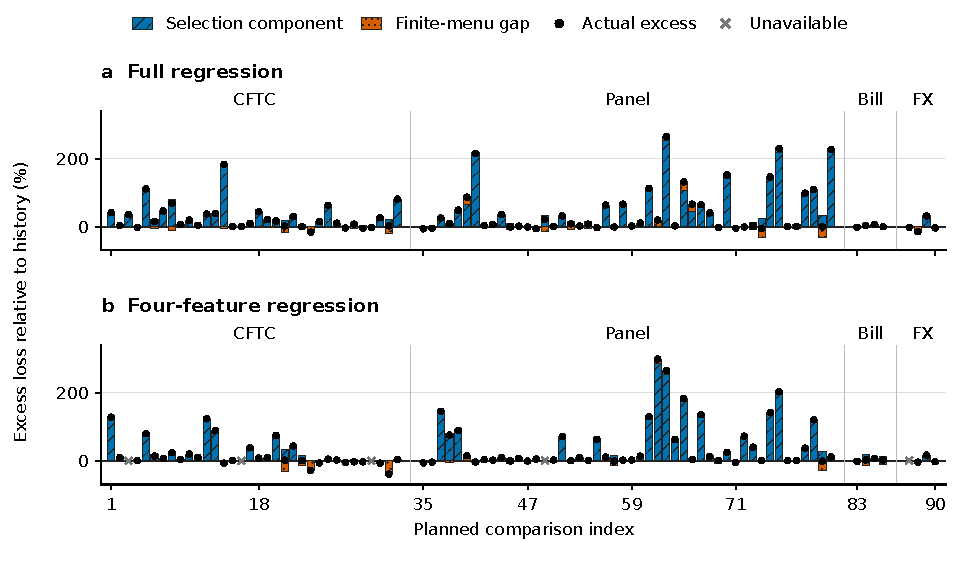
\includegraphics[width=.98\linewidth]{figures/v12-decomposition.pdf}
\caption{Signed decomposition of regression excess loss against matched historical headroom, with selection in blue, the finite-menu diagnostic gap in orange, and actual excess as black dots. Crosses retain unavailable comparisons; the text focuses on short-history weekly cells while all planned comparisons remain plotted. The weekly comparisons retain both selection losses and a remaining gap within the tested menu, so hindsight selection alone need not recover historical performance.}\label{fig:v12-decomposition}
\end{figure}

Extending validation from 52 to 156 weeks keeps the CFTC evaluation period, training histories and refitting clock fixed in the saved sensitivity exercise.
Consider first the 52-week training history, which retains its own historical reference and forecast dates when the validation period is extended.
Its median excess falls from 19.33\% to 4.03\%, showing a narrower loss disadvantage under the longer validation period in this comparison.

For the 260-week training history, the same exercise again holds the evaluated targets, historical benchmark and refitting schedule fixed.
Its median excess falls from 10.35\% to 0.53\%, while the complete results retain the variation among contracts around these separate medians.

Infinite-penalty selections rise from 4 to 10 contracts under the shorter training history, favoring the ordinary empirical quantile more often.
Under the longer training history, these selections rise from 4 to 5 contracts, again retaining the full market universe in the denominator.
Each comparison covers 17 contracts; differences between their separate medians leave typical paired improvements and a causal interpretation unresolved.
Four-feature failures remain unavailable in the complete inventory, preserving the distinction between a successful subset and its planned comparison (Supplement Section S15).

Tail-level sensitivity remains incomplete, as the retained supplementary tail-sensitivity table shows for 90\% and 99\% quantiles under matched histories. Consider the 99\% target separately, retaining the originally planned comparisons and the numerical failure recorded under that quantile sensitivity design.
Historical headroom wins 28 of 34 CFTC comparisons, while the remaining numerical failure prevents classification of the complete planned group.
The registered threshold requires 29 wins, leaving its verdict unresolved until the failed comparison can be determined under an authorized analysis.
Both FX periods remain unavailable at 99\%, leaving the combined improvement criterion undetermined and their failed planned comparisons explicitly retained.
Successful subsets remain distinct from a missing full-group median, preserving the original uncertainty instead of replacing it with a favorable partial summary.




\subsection{Scores and breach behavior answer different questions}

Accuracy rankings leave breach behavior unresolved: the matched FX gain coexists with more breaches before calibration (Table~\ref{tab:fx}). Pinball loss measures error amounts while a strict-hit indicator records event occurrence, so monitoring reports should show both forms of error.

Elementary-score rankings cross for both original main comparisons (\href{https://github.com/ByronLi0207/financial-mathematics-paper-20261020/blob/final-jof/EXTENDED_RESULTS.md}{the original full Supplement: Figures S2--S3}, \href{https://github.com/ByronLi0207/financial-mathematics-paper-20261020/blob/final-jof/EXTENDED_RESULTS.md}{the original full Supplement: Section S33}). A separate 24-step FX comparison against rolling translated paths changes ranking as the relative penalty on underprediction rises across the evaluated preferences.
Its reversal occurs near 20.6:1, reflecting the weighting of underprediction against overprediction in that particular comparison of the saved reports.
Both six-step FX comparisons reduce mean underprediction and mean overprediction, confining this weight reversal to the longer-horizon translated-path reference.

Loss and hit diagnostics answer different questions (\href{https://github.com/ByronLi0207/financial-mathematics-paper-20261020/blob/final-jof/EXTENDED_RESULTS.md}{the original full Supplement: Table S47}, \href{https://github.com/ByronLi0207/financial-mathematics-paper-20261020/blob/final-jof/EXTENDED_RESULTS.md}{the original full Supplement: Section S33}). HAC tests compare average loss and strict-hit tests examine event frequency and serial behavior, while RMS-state diagnostics compare conditional predictive ability across training-defined groups \citep{gw2006}.

\FloatBarrier


\section{Why history length matters}\label{sec:history-mechanism}

\subsection{A descriptive ratio organizes the simulation evidence}

Let the training history contain $W$ completed targets and let the horizon span
$H$ subsequent observations. The earlier discovery study selected the following ratio as a descriptive coordinate on its fixed simulation grid, leaving model complexity outside its definition:
\[
c=\frac{W}{H+1}.
\]
It excludes the number of coefficients, so an interpretation as dependence-adjusted information or an identified complexity normalization remains unsupported by this design. Estimating a
separate threshold for each method also makes a later constant rescaling within
that method observationally equivalent for the history-region checks.

The discovery first crossing is approximately $106.5$ for full regression, locating the initial change in sign on the selected simulation coordinate.
For the sparse regression it is approximately $27.3$, with the underlying curve retaining further changes in direction across the tested grid.
The full-regression fixed-grid interval runs from $27.89$ to $110.71$, summarizing the original resampling uncertainty conditional on the selected coordinate.
The sparse-regression interval runs from $13.27$ to $107.11$, under the same restriction to the selected coordinate and simulation grid.
Uncertainty from choosing that coordinate remains outside these ranges, and repeated downward crossings invalidate a permanently sufficient history interpretation.

The subsequent registered simulation checks meet the short-history prediction in $47$ of $48$ cells under the declared simulation laws and menus.
The long-history prediction holds in $21$ of $24$ cells, retaining the exceptions and the original fixed denominators in its descriptive count.
These are finite-grid descriptive successes rather than independent-cell significance tests, because the experiments share their designed laws and comparison structure.
The simpler procedure satisfies the universal-ordering inequality in $42$ of $48$ cells, falling short of the all-cell requirement for that claim.
All six counterexamples remain in the evidence, so the universal simplification claim fails despite its inequality holding across most tested cells.

\subsection{FX curves retain left censoring and long-history reversals}

Figure~\ref{fig:history} retains both regression variants and both FX horizons,
alongside the earlier simulation and financial comparisons. Three identified
financial first crossings fall within the broad transported ranges. Another
curve already favors regression at its shortest tested history, leaving its
first crossing left-censored. A pooled simulation crossing and a crossing at
one fixed financial horizon are different objects. Their agreement leaves a horizon-invariant financial threshold unidentified, since the transported simulation summary and the individual financial curve represent different objects.

Both longer-horizon FX curves lose their advantage again at the largest
history. The shorter-horizon full-regression gain also weakens after its best
tested history. These are the previously studied FX observations, including
overlap with earlier comparisons. Their reuse supports a within-record history comparison, leaving replication across individual dealers and validation on an untouched financial holdout unresolved.

\begin{figure}[p]\centering
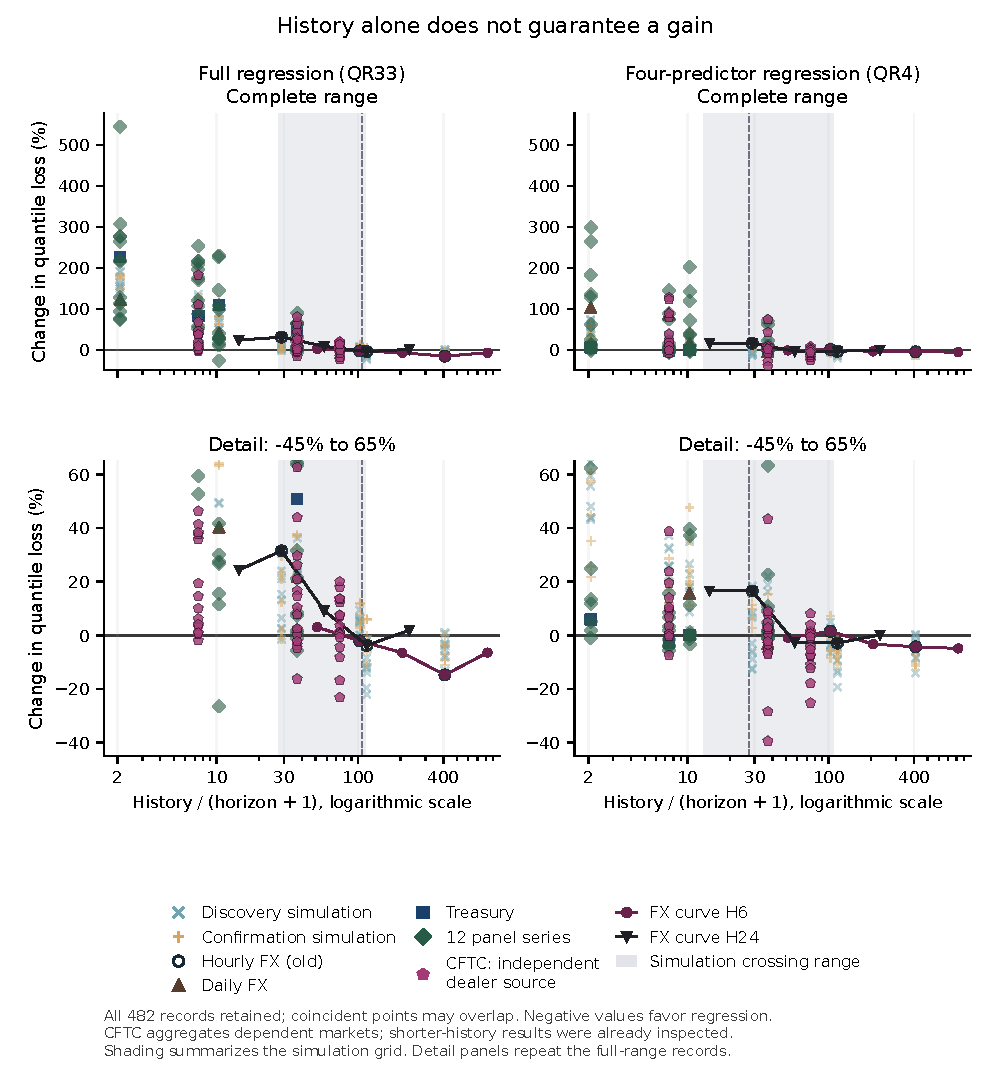
\includegraphics[width=.98\linewidth,height=.78\textheight,keepaspectratio]{figures/final-unified-history.pdf}
\caption{All earlier conditional-model records and all CFTC comparisons are retained against their own matched historical benchmark. Negative changes favor regression. The upper panels preserve the complete range; the lower panels repeat the same records in a labelled detail range. Eight FX records reuse an earlier period. CFTC is an independent reporting source of aggregate, potentially dependent markets; its shorter-history outcomes were already inspected. Shading summarizes the original simulation crossings conditional on the chosen grid and coordinate, with uncertainty from selecting that coordinate omitted.
History alone leaves gains unguaranteed, as the complete curves retain adverse comparisons, left censoring and reversals at the longest histories.}\label{fig:history}
\end{figure}

\subsection{CFTC meets the short-history count but misses the long-history target}

The CFTC extension fixes the earlier thresholds before adding a training history of $520$ weeks, while reusing the unchanged shorter-history reports.
The universe, validation period, evaluation dates, candidate menus and refit schedule remain inherited, confining the new computation to the registered extension.
Its protocol was locally committed before the new fits, while shorter-history outcomes were already known and external public preregistration remains unclaimed.
The candidate menus differ from the simulation discovery menus, making this a transported prediction check rather than a replication with identical procedures.
Training labels have completed by each refit and every validation label finishes before evaluation, under the stipulated downloaded economic-date information convention.
Historical first-release information remains distinct and unreconstructed, preserving the difference between a valid completed-label schedule and actual public availability.

For the full procedure, the low-history region contains $34$ planned market-history comparisons, all retained under the registered classification and denominator.
It loses to matched historical headroom in $29$ comparisons, meeting the registered disadvantage criterion within this low-history region of the grid.
The sparse procedure loses in $15$ of $17$ low-history comparisons, retaining the same fixed historical reference in each paired comparison.
Both meet their registered eighty-percent targets, supporting the short-history sign pattern under these particular menus and transported simulation thresholds.

The sparse procedure wins in $10$ of $17$ long-history markets, leaving a substantial set of adverse contracts in the same region.
That fraction misses its registered sixty-percent target, making the primary verdict partial agreement despite the successful short-history disadvantage counts.

Only $6$ of $17$ sparse-regression curves improve strictly at both steps of the history grid, retaining every reversal or tie.
This misses the secondary seventy-percent target, which remains separate from the primary verdict and preserves the failure of strict improvement.

\begin{table}[htbp]\centering\small
\caption{Registered CFTC history-region predictions. The primary verdict is partial agreement because both short-history screens pass and the sparse long-history screen fails.}\label{tab:cftc-mechanism}
\begin{tabular}{lllll}\toprule
Prediction & Procedure & Region / ordering & Successes & Verdict\\\midrule
P1 & Full regression & $c<r^*/2$ & $29/34$ & Supported\\
P1 & Four predictors & $c<r^*/2$ & $15/17$ & Supported\\
P2 & Four predictors & $c>2r^*$ & $10/17$ & Not supported\\
P2 & Full regression & No eligible high-region cell & NA & Not testable\\
P3 & Four predictors & Strict fall at both history steps & $6/17$ & Not supported\\
\bottomrule\end{tabular}
\par\smallskip\begin{minipage}{.98\linewidth}\footnotesize
Both P1 screens must pass; the primary verdict then combines P1 and sparse P2.
P3 is secondary and leaves that verdict unchanged; ties enter a separate category outside both the win and loss counts.
Unknowns retain planned denominators under the registered classification bounds, although all planned reports complete in this particular run.
All comparisons use matched corrected-rank F, rather than selecting the better
of F and I after evaluation. Both model procedures can select ordinary I.
\end{minipage}\end{table}

Seven markets remain adverse for the sparse procedure at the long history.
The complete market-level scores, strict breaches, HAC diagnostics and
counterexamples remain in the supplementary result inventory and linked source
tables. The primary verdict retains every market, failed criterion and unfavorable curve, with the full denominators fixed by the registered design. The shorter CFTC outcomes were known before this
registration, so the extension is prospective only for its new computations.
It gives partial agreement with a transported pattern, rather than a complete
independent confirmation or causal identification of estimation cost.

\FloatBarrier

\section{Limit-cost rankings depend on the stated charges}\label{sec:cost}

\[
J_m(\kappa,\beta,c)=\kappa\frac{\overline{C_m-B}}{m_F}
+\beta\,\overline{\mathbf 1\{Y>C_m\}}
+c\frac{\overline{(Y-C_m)_+}}{m_F},\qquad
m_F=\overline{C_F-B}>0,\quad\beta=b/m_F.
\]

For CFTC full regression, higher reserve coefficients and lower fixed-breach coefficients generally favor the expanded-menu procedure, although the fixed grid retains local reversals (Figure~\ref{fig:decision}).
The exceedance-magnitude coefficient is fixed at $c=1$, separating this charge from the reserve and breach-event preferences varied across the grid.

At the center of the sorted grid, the reserve and breach-event coefficients are $(\kappa,\beta)=(.1,.25)$ under the stated normalization.
Regression is strictly cheaper in $5/34$ comparisons there, retaining the same matched historical report and the original histories for each contract.

At the reserve-heavy corner the coefficients are $(1,0)$, so reserve amounts and exceedance magnitude entirely determine these illustrative costs.
Regression is cheaper in $32/34$ comparisons there, illustrating how a different balance of stated costs can change the preferred report.

At the opposite corner the coefficients are $(.01,5)$, placing greater weight on breach events relative to the reported reserve amount.
Regression is cheaper in $1/34$ comparisons there, with the complete grid retaining the intervening outcomes and any local exceptions.

These costs express hypothetical preferences rather than observed operating expenses, and Supplement Section S12 retains their normalization and complete-method results.
Each contract uses its own historical headroom scale, so these normalized comparisons leave common-dollar costs and a common exposure measure unidentified.

\begin{figure}[htbp]\centering
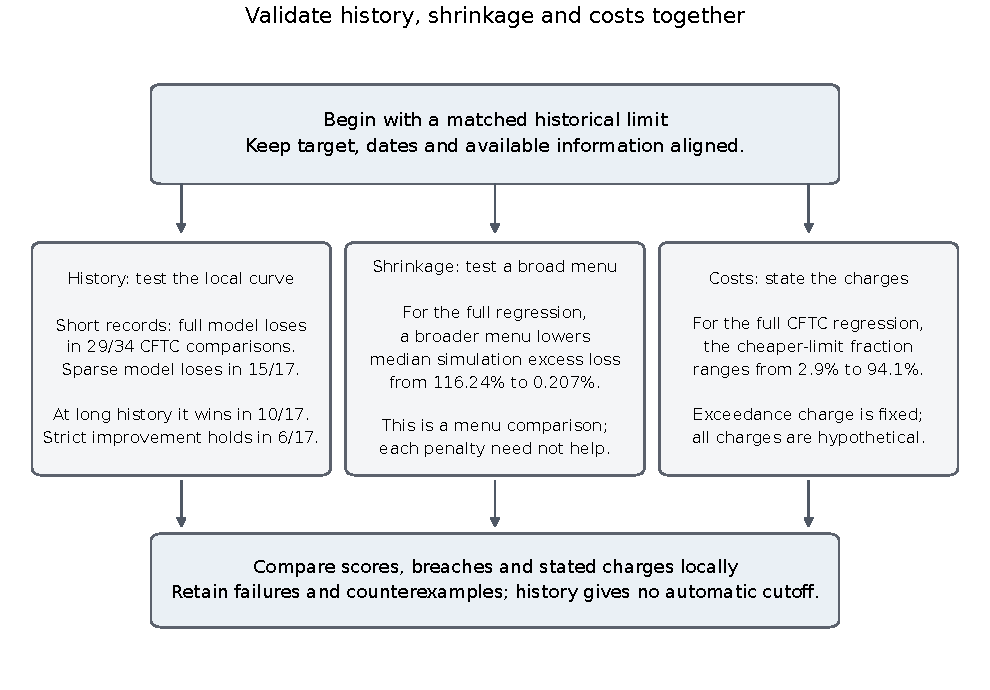
\includegraphics[width=.98\linewidth]{figures/final-decision-map.pdf}
\caption{History, the tested penalty menu and stated cost preferences guide a matched comparison. The simulation median is full regression at the shorter history in the constant-parameter experiment. The CFTC cost fraction refers only to full regression at the original histories, varying reserve and breach-event charges with the exceedance-magnitude charge fixed. All charges are hypothetical. History, shrinkage and stated costs must be assessed together in the intended application.}\label{fig:decision}
\end{figure}

\FloatBarrier

\section{Implications for model validation}\label{sec:implications}

\textbf{Benchmark against historical headroom.} Use the same completed labels, history length and refit schedule, naming the shorter rolling reference separately because its FX ranking changes across periods. This keeps differences in available history distinct from the gains associated with conditioning within a matched comparison.

\textbf{Retain historical headroom as a demanding validation benchmark.} Expanded penalties and longer validation reduce losses, but short-sample selection, including one-standard-error selection, still fails to protect the historical benchmark consistently. Historical reports also survive in most CFTC model confidence sets, supporting their retention as benchmarks while a conditional procedure undergoes application-specific validation. The ordinary empirical quantile is up to 36.5\% worse than corrected headroom in the earlier weekly grid.

\textbf{Report breaches with the score.} Show mean underprediction, mean overprediction and strict-breach counts together, since the unwrapped matched FX gain and daily regression exception both accompany more breaches than history. Cost regions add reserve, breach-frequency and exceedance preferences to this joint evaluation.

\FloatBarrier

\section{Limitations}\label{sec:limitations}

\begin{itemize}\setlength{\itemsep}{0pt}\setlength{\parskip}{0pt}
\item FX comes from one market maker, and its original evaluation period was inspected before conditional methods were specified.
\item The earlier-period comparison and full-prefix backcast are retrospective, leaving a previously unseen prospective financial evaluation outside the completed evidence.
\item Weekly reports aggregate positions across dealers, making related categories and the CFTC survivor universe comparisons of reporting aggregates rather than independent dealer replications.
\item Downloaded economic-date vintages omit historical first-release information and reporting delays, keeping the retrospective position clock distinct from public information availability.
Sampled net positions can miss within-interval excursions and gross dealer exposure; daily final records are observed timestamps rather than verified market closes.
\item Causal effects, individual-feature effects and coverage guarantees remain unidentified by these dependent forecast comparisons, even when completed training-label histories match.
\item Costs illustrate fixed preferences under the recorded position paths, leaving trading returns, funding gains and institutional intervention costs unmeasured by these experiments.
\item Choosing the best finite candidate after evaluation is diagnostic only; validation-length and quantile-sensitivity checks are post-result analyses with numerical failures retained.
\end{itemize}
Supplement Section S15 retains the original technical qualifications on simulations, aggregation and forecast comparison.

\FloatBarrier

\section{Conclusion}\label{sec:conclusion}

Historical rules are hard to beat in these position records. Matched FX gains
coexist with adverse daily and weekly comparisons, changing reference rankings
and nonmonotone history curves. The original evaluation period was inspected, and related reporting categories remain aggregate comparisons with individual-dealer replication outside their scope.

The history evidence supports a bounded interpretation. Registered simulations
meet the short-history and long-history loss-sign criteria, while their
universal simplification claim fails. The CFTC extension gives partial
agreement: short-history disadvantage counts pass, whereas the long-history
win target and strict-improvement target fail. An automatic deployment rule based only on longer history therefore remains unsupported by these completed comparisons and their retained exceptions.

The menu and selection evidence complements that result. A broader simulated
menu reduces a large short-history disadvantage, but the available financial
menu and its selection procedure still leave losses. Access to a historical candidate leaves predictor value unidentified by menu expansion alone, since near-parity can result from selecting that historical option. The high-quantile failures remain unavailable and prevent a general
extension of the original gains to the higher target level.

Reserve amounts, breach frequency and exceedance magnitude also affect the
preferred tested report under stated charges. The fixed cost grids have local
exceptions and express hypothetical preferences, rather than realized trading
or funding benefits. Validation should retain a matched historical benchmark,
display the complete history sensitivity and report all three cost components
alongside scores and failures. Figure~\ref{fig:decision} summarizes this bounded
evaluation guidance.

\FloatBarrier

\section*{Data and code availability}
\paragraph{Data availability.} The FX input is the specified version of the Kaggle Net Position Time Series Dataset. The owning metadata labels its license ``Data files \copyright\ Original Authors.'' This repository supplies the acquisition route and input fingerprint, but excludes raw FX observations and private per-issue prediction vectors. Obtain the source from \url{https://www.kaggle.com/datasets/davidlindsay1979/net-position-time-series-dataset} subject to the original rights holders' terms.

The New York Fed aggregates are available from its Primary Dealer Statistics service under the Bank's Terms of Use. The repository preserves the unchanged accepted Treasury snapshot with attribution and identifies study calculations separately. Copying or distributing that content remains subject to its source notices, attribution, modification labeling, continuing conditions and endorsement restrictions: \url{https://www.newyorkfed.org/privacy/termsofuse.html}. The code license does not replace those source conditions.

The CFTC application uses the public TFF historical files from \url{https://www.cftc.gov/MarketReports/CommitmentsofTraders/HistoricalCompressed/index.htm}. The repository includes unchanged downloaded archives and a per-file URL, acquisition time, byte count and SHA-256 record in \texttt{data/cftc-tff/provenance.json}.

\paragraph{Code availability.} Code, results and reproduction instructions are available at \url{https://github.com/ByronLi0207/financial-mathematics-paper-20261020/tree/final-jof}.

\section*{Author-provided information}
Author information: [TO BE COMPLETED BY AUTHOR].\par
ORCID: [TO BE COMPLETED BY AUTHOR].\par
Funding: [TO BE COMPLETED BY AUTHOR].\par
Competing interests: [TO BE COMPLETED BY AUTHOR].\par

\begin{thebibliography}{99}
\raggedright
\bibitem[Arjani et al.(2020)]{arjani2020} Arjani, N., Li, F., \& Sabetti, L. (2020). \emph{Monitoring intraday liquidity risks in a real time gross settlement system}. Payments Canada. \url{https://www.payments.ca/sites/default/files/discussion_paper_monitoring_intraday_liquidity_risks_in_a_real_time_gross_settlement_system.pdf}

\bibitem[Avellaneda \& Stoikov(2008)]{avellaneda2008} Avellaneda, M., \& Stoikov, S. (2008). High-frequency trading in a limit order book. \emph{Quantitative Finance}, \emph{8}(3), 217--224. \url{https://doi.org/10.1080/14697680701381228}

\bibitem[Barone-Adesi et al.(1999)]{barone1999} Barone-Adesi, G., Giannopoulos, K., \& Vosper, L. (1999). VaR without correlations for portfolios of derivative securities. \emph{Journal of Futures Markets}, \emph{19}(5), 583--602. \url{https://doi.org/10.1002/(SICI)1096-9934(199908)19:5<583::AID-FUT5>3.0.CO;2-S}

\bibitem[Board of Governors of the Federal Reserve System(2013)]{fr2004_2013} Board of Governors of the Federal Reserve System. (2013, March). \emph{Reporting guidelines for preparing the FR 2004 primary government securities dealers reports}. \url{https://www.federalreserve.gov/apps/reportingforms/Download/DownloadAttachment?guid=f555fe11-e149-479b-8088-4ed4e9ae1206}

\bibitem[Board of Governors of the Federal Reserve System(2024)]{fr2004_2024} Board of Governors of the Federal Reserve System. (2024, July). \emph{Instructions for the preparation of government securities dealers reports: Reporting form FR 2004}. \url{https://www.federalreserve.gov/apps/reportingforms/Download/DownloadAttachment?guid=950ab256-b485-4586-99b0-b27eb205fdfa}

\bibitem[Bollerslev(1986)]{bollerslev1986} Bollerslev, T. (1986). Generalized autoregressive conditional heteroskedasticity. \emph{Journal of Econometrics}, \emph{31}(3), 307--327. \url{https://doi.org/10.1016/0304-4076(86)90063-1}

\bibitem[Boudoukh et al.(2004)]{boudoukh2004} Boudoukh, J., Richardson, M., Stanton, R., \& Whitelaw, R. F. (2004). MaxVaR: Long-horizon value at risk in a mark-to-market environment. \emph{Journal of Investment Management}, \emph{2}(3), 1--6. \url{https://pages.stern.nyu.edu/~rwhitela/papers/maxvar%20joim04.pdf}

\bibitem[Christoffersen(1998)]{christ1998} Christoffersen, P. F. (1998). Evaluating interval forecasts. \emph{International Economic Review}, \emph{39}(4), 841--862. \url{https://doi.org/10.2307/2527341}

\bibitem[Commodity Futures Trading Commission(n.d.)]{cftcTFF} Commodity Futures Trading Commission. (n.d.). \emph{Historical compressed}. Retrieved October 24, 2026, from \url{https://www.cftc.gov/MarketReports/CommitmentsofTraders/HistoricalCompressed/index.htm}

\bibitem[Diebold \& Mariano(1995)]{dm1995} Diebold, F. X., \& Mariano, R. S. (1995). Comparing predictive accuracy. \emph{Journal of Business \& Economic Statistics}, \emph{13}(3), 253--263. \url{https://doi.org/10.1080/07350015.1995.10524599}

\bibitem[Duffie et al.(2023)]{duffie2023} Duffie, D., Fleming, M. J., Keane, F. M., Nelson, C., Shachar, O., \& Van Tassel, P. (2023). \emph{Dealer capacity and U.S. Treasury market functionality} (Staff Report No. 1070, August; revised October). Federal Reserve Bank of New York Staff Reports. \url{https://doi.org/10.59576/sr.1070}

\bibitem[Ehm et al.(2016)]{ehm2016} Ehm, W., Gneiting, T., Jordan, A., \& Krüger, F. (2016). Of quantiles and expectiles: Consistent scoring functions, Choquet representations and forecast rankings. \emph{Journal of the Royal Statistical Society Series B: Statistical Methodology}, \emph{78}(3), 505--562. \url{https://doi.org/10.1111/rssb.12154}

\bibitem[Engle \& Manganelli(2004)]{engle2004} Engle, R. F., \& Manganelli, S. (2004). CAViaR: Conditional autoregressive value at risk by regression quantiles. \emph{Journal of Business \& Economic Statistics}, \emph{22}(4), 367--381. \url{https://doi.org/10.1198/073500104000000370}

\bibitem[Federal Reserve Bank of New York(n.d.)]{nyfeddata} Federal Reserve Bank of New York. (n.d.). \emph{Primary dealer statistics} [Data set]. Retrieved October 23, 2026, from \url{https://www.newyorkfed.org/markets/counterparties/primary-dealers-statistics}

\bibitem[Giacomini \& White(2006)]{gw2006} Giacomini, R., \& White, H. (2006). Tests of conditional predictive ability. \emph{Econometrica}, \emph{74}(6), 1545--1578. \url{https://doi.org/10.1111/j.1468-0262.2006.00718.x}

\bibitem[Gibbs \& Candès(2021)]{gibbs2021} Gibbs, I., \& Candès, E. J. (2021). Adaptive conformal inference under distribution shift. In M. Ranzato, A. Beygelzimer, Y. Dauphin, P. S. Liang, \& J. Wortman Vaughan (Eds.), \emph{Advances in Neural Information Processing Systems} (Vol. 34, pp. 1660--1672). Curran Associates, Inc. \url{https://proceedings.neurips.cc/paper_files/paper/2021/hash/0d441de75945e5acbc865406fc9a2559-Abstract.html}

\bibitem[Gneiting(2011)]{gneiting2011} Gneiting, T. (2011). Making and evaluating point forecasts. \emph{Journal of the American Statistical Association}, \emph{106}(494), 746--762. \url{https://doi.org/10.1198/jasa.2011.r10138}

\bibitem[Hansen(1992)]{hansen1992} Hansen, B. E. (1992). Testing for parameter instability in linear models. \emph{Journal of Policy Modeling}, \emph{14}(4), 517--533. \url{https://doi.org/10.1016/0161-8938(92)90019-9}

\bibitem[Hansen et al.(2011)]{mcs2011} Hansen, P. R., Lunde, A., \& Nason, J. M. (2011). The model confidence set. \emph{Econometrica}, \emph{79}(2), 453--497. \url{https://doi.org/10.3982/ECTA5771}


\raggedright

\bibitem[Harvey et al.(1997)]{hln1997} Harvey, D., Leybourne, S., \& Newbold, P. (1997). Testing the equality of prediction mean squared errors. \emph{International Journal of Forecasting}, \emph{13}(2), 281--291. \url{https://doi.org/10.1016/s0169-2070(96)00719-4}

\bibitem[Hastie et al.(2009)]{hastie2009} Hastie, T., Tibshirani, R., \& Friedman, J. (2009). \emph{The elements of statistical learning: Data mining, inference, and prediction} (2nd ed.). Springer. \url{https://doi.org/10.1007/978-0-387-84858-7}

\bibitem[Holm(1979)]{holm1979} Holm, S. (1979). A simple sequentially rejective multiple test procedure. \emph{Scandinavian Journal of Statistics}, \emph{6}(2), 65--70. \url{https://www.jstor.org/stable/4615733}

\bibitem[Hull \& White(1998)]{hull1998} Hull, J., \& White, A. (1998). Incorporating volatility updating into the historical simulation method for value-at-risk. \emph{The Journal of Risk}, \emph{1}(1), 5--19. \url{https://doi.org/10.21314/jor.1998.001}

\bibitem[Koenker \& Bassett(1978)]{koenker1978} Koenker, R., \& Bassett, G., Jr. (1978). Regression quantiles. \emph{Econometrica}, \emph{46}(1), 33--50. \url{https://doi.org/10.2307/1913643}

\bibitem[Kupiec(1995)]{kupiec1995} Kupiec, P. H. (1995). Techniques for verifying the accuracy of risk measurement models. \emph{The Journal of Derivatives}, \emph{3}(2), 73--84. \url{https://doi.org/10.3905/jod.1995.407942}

\bibitem[Lindsay(2020)]{dataset} Lindsay, D. (2020). \emph{Net position time series dataset} (Version 2) [Data set]. Kaggle. \url{https://www.kaggle.com/datasets/davidlindsay1979/net-position-time-series-dataset}

\bibitem[McNeil \& Frey(2000)]{mcneilfrey2000} McNeil, A. J., \& Frey, R. (2000). Estimation of tail-related risk measures for heteroscedastic financial time series: An extreme value approach. \emph{Journal of Empirical Finance}, \emph{7}(3--4), 271--300. \url{https://doi.org/10.1016/s0927-5398(00)00012-8}

\bibitem[Meinshausen(2006)]{meinshausen2006} Meinshausen, N. (2006). Quantile regression forests. \emph{Journal of Machine Learning Research}, \emph{7}(35), 983--999. \url{https://www.jmlr.org/papers/v7/meinshausen06a.html}

\bibitem[Newey \& West(1987)]{nw1987} Newey, W. K., \& West, K. D. (1987). A simple, positive semi-definite, heteroskedasticity and autocorrelation consistent covariance matrix. \emph{Econometrica}, \emph{55}(3), 703--708. \url{https://doi.org/10.2307/1913610}

\bibitem[Petrunia et al.(2019)]{petrunia2019} Petrunia, R., Sabetti, L., \& Voia, M. (2019). \emph{Tail risk in the automated clearing settlement system (ACSS)} (Discussion Paper No. 7). Payments Canada. \url{https://www.payments.ca/sites/default/files/tail_risk_in_the_automated_clearing_settlement_system_acss.pdf}

\bibitem[van den Hoogen(2017)]{hoogen2017} van den Hoogen, S. (2017). \emph{Intraday liquidity risk estimation using transaction data: An extreme value theory approach} [Master's thesis, Delft University of Technology]. TU Delft Repository. \url{https://resolver.tudelft.nl/uuid:1c0c4545-bb07-4916-aa37-1d4bea3b7872}

\bibitem[Wisniewski et al.(2020)]{wisniewski2020} Wisniewski, W., Lindsay, D., \& Lindsay, S. (2020). Application of conformal prediction interval estimations to market makers' net positions. In A. Gammerman, V. Vovk, Z. Luo, E. Smirnov, \& G. Cherubin (Eds.), \emph{Proceedings of the Ninth Symposium on Conformal and Probabilistic Prediction and Applications} (Proceedings of Machine Learning Research, Vol. 128, pp. 285--301). PMLR. \url{https://proceedings.mlr.press/v128/wisniewski20a.html}

\bibitem[Wisniewski(2024)]{wisniewski2024} Wisniewski, W. J. (2024). \emph{Net position and retail trader behaviour: Implications for market makers' risk management strategies} [Doctoral dissertation, Royal Holloway, University of London]. Royal Holloway Research Portal. \url{https://pure.royalholloway.ac.uk/en/publications/net-position-and-retail-trader-behaviour-implications-for-market-/}
\end{thebibliography}

\end{document}
